\chapter{Analisis}
\label{chap:analisis}

\section{Analisis Sistem Kini}
\label{sec:analisissistemkini}
Berikut adalah penjelasan secara umum mengenai Kode KIRI (gambar \ref{fig:3_strukturkiri}):
\begin{enumerate}
	\item \textit{Folder} ``.settings'' merupakan \textit{folder} yang menyimpan \textit{file-file} pengaturan kode KIRI untuk Eclipse.
	\item \textit{Folder} ``etc'' merupakan \textit{folder} yang menyimpan \textit{file-file} untuk membangun konstanta-konstanta dan fungsi-fungsi yang digunakan oleh sistem KIRI.
	\item \textit{Folder} ``log'' merupakan \textit{folder} yang berisi \textit{file-file} untuk mencatat setiap kinerja sistem KIRI.
	\item \textit{Folder} ``public\_html'' merupakan \textit{folder} yang berisi \textit{file-file} untuk membangun KIRI \textit{Front End}.
	\item \textit{Folder} ``public\_html\_dev'' merupakan \textit{folder} yang berisi \textit{file-file} untuk membangun KIRI \textit{Dashboard}.
	\item \textit{Folder} ``res'' merupakan \textit{folder} yang berisi \textit{file-file} yang bersifat publik seperti gambar dan XML yang digunakan sebagai pendukung sistem KIRI.
	\item \textit{Folder} ``sql'' merupakan \textit{folder} yang menyimpan \textit{database} sistem KIRI.
\end{enumerate}

\begin{figure}[htbp]
	\centering
		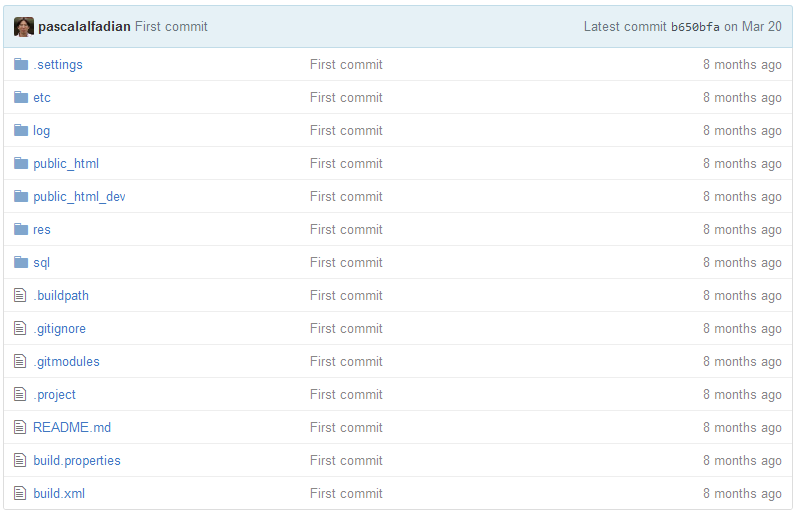
\includegraphics[scale=0.5]{Gambar/3_strukturkiri.png}
	\caption{Struktur Kode KIRI}
	\label{fig:3_strukturkiri}
\end{figure}

\begin{figure}[htbp]
	\centering
		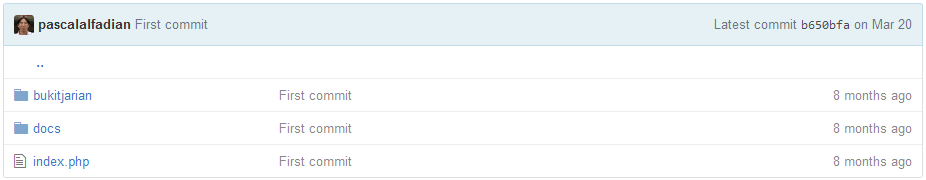
\includegraphics[scale=0.5]{Gambar/3_public_html_dev.png}
	\caption{Struktur \textit{folder} ``public\_html\_dev''}
	\label{fig:3_public_html_dev}
\end{figure}

\begin{figure}[htbp]
	\centering
		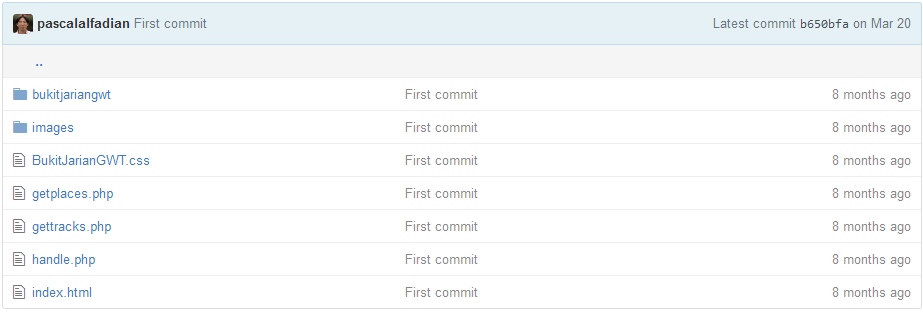
\includegraphics[scale=0.5]{Gambar/3_bukit_jarian.png}
	\caption{Struktur \textit{folder} ``bukitjarian''}
	\label{fig:3_bukit_jarian}
\end{figure}

\begin{figure}[htbp]
	\centering
		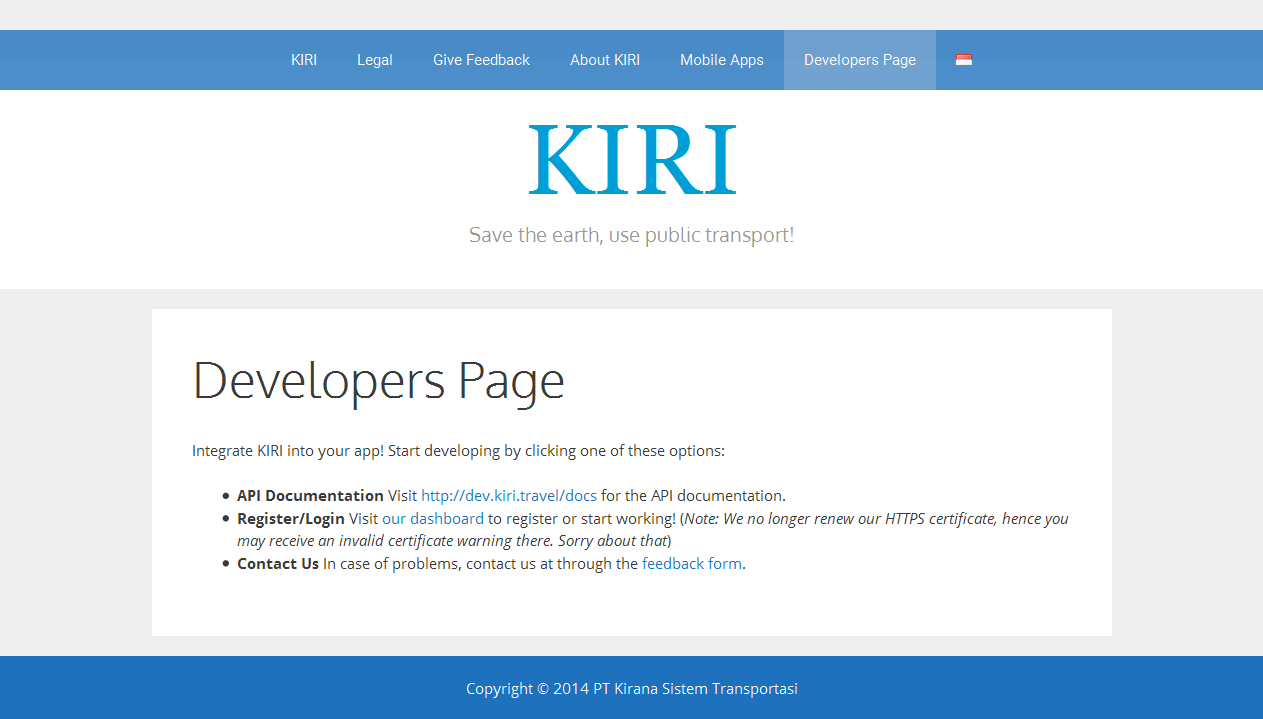
\includegraphics[scale=0.35]{Gambar/3_developer.png}
	\caption{Halaman developer KIRI}
	\label{fig:3_developer}
\end{figure}

\begin{figure}[htbp]
	\centering
		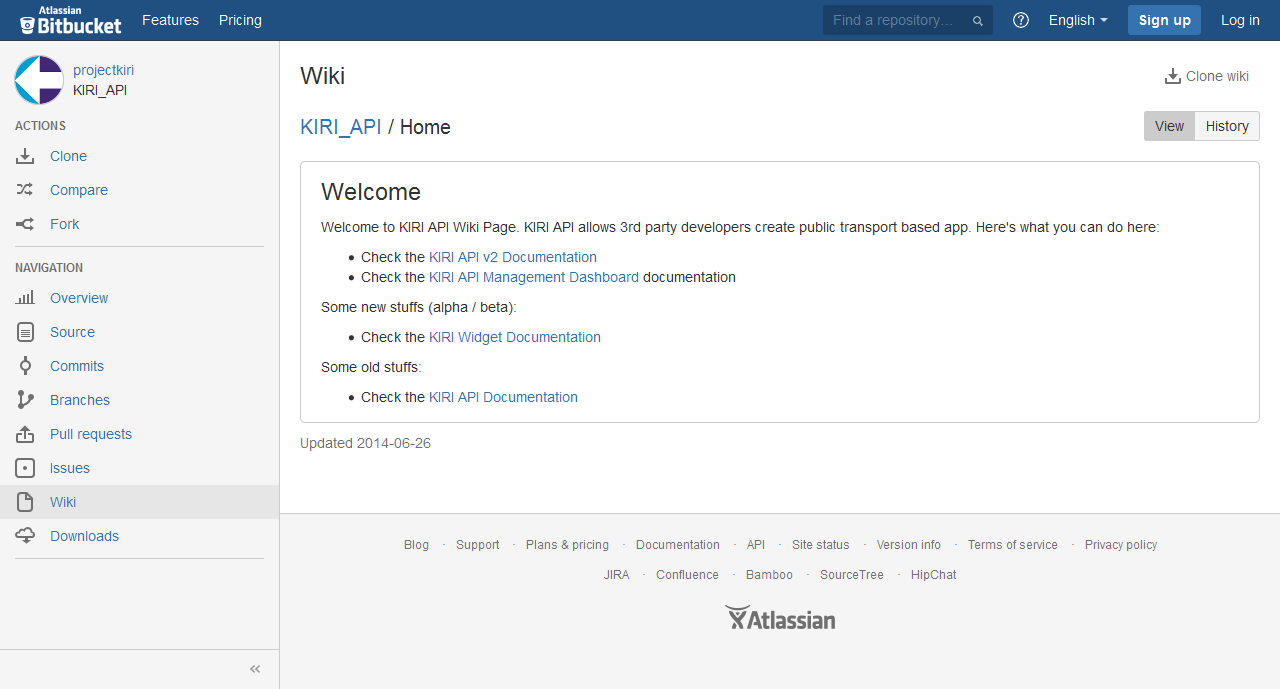
\includegraphics[scale=0.35]{Gambar/3_dokumentasi.png}
	\caption{Halaman dokumentasi KIRI}
	\label{fig:3_dokumentasi}
\end{figure}

Penelitian ini berfokus pada pembahasan KIRI \textit{Dashboard}, untuk itu bagian yang akan dibahas lebih mendalam adalah hanya bagian ``public\_html\_dev'' (gambar \ref{fig:3_public_html_dev}) dan beberapa bagian-bagian pendukung untuk membangun KIRI \textit{Dashboard}. \textit{Folder} ``public\_html\_dev'' memiliki struktur sebagai berikut:
\begin{enumerate}
	\item \textit{Folder} ``bukitjarian'', berisi mengenai \textit{file-file} untuk membangun KIRI \textit{Dashboard} (gambar \ref{fig:3_bukit_jarian}).
	\item \textit{Folder} ``docs'', berisi mengenai \textit{file-file} yang akan mengarahkan ke bagian dokumentasi KIRI (gambar \ref{fig:3_dokumentasi}).
	\item ``index.php'', bila \textit{file} ini dieksekusi maka akan mengarahkan pengguna ke halaman developer KIRI (gambar \ref{fig:3_developer}), dimana berisi informasi mengenai alamat KIRI \textit{Dashboard}, dokumentasi KIRI, dan halaman untuk memberikan \textit{feedback}.
\end{enumerate}

Pada direktori ``public\_html\_dev/bukitjarian'' (gambar \ref{fig:3_bukit_jarian}) terdapat bermacam-macam \textit{file} dan \textit{folder}. Berdasarkan wawancara dengan kontributor kode, terdapat dua bagian \textit{file} dan \textit{folder} yang berperan penting dalam membangun KIRI \textit{Dashboard}:
\begin{enumerate}
	\item ``index.html'', ``bukitjariangwt/'', dan ``images/''. \textit{File} dan \textit{folder} ini dibangun dengan menggunakan perangkat lunak GWT. GWT berguna untuk melakukan konversi kode dalam bahasa Java menjadi HTML dan JavaScript. Hasil konversi menggunakan GWT akan mengalami \textit{obfuscate} (pengacakan) sehingga sulit untuk dianalisa. Namun demikian, \textit{file-file} ini bersifat statis dan tidak memerlukan operasi khusus di \textit{server}, sehingga dapat disalin (\textit{copy}) apa adanya. 
	\item ``handle.php'' merupakan kode pada sisi \textit{server} yang bertugas untuk melayani permintaan-permintaan dari \textit{browser} yang dieksekusi oleh ``index.html''.
\end{enumerate}

Seperti disebutkan sebelumnya, \textit{file} ``handle.php'' berfungsi untuk melayani permintaan-permintaan yang dikirimkan oleh ``index.html''. \textit{File} ini dapat dibagi menjadi 16 bagian yang masing-masing melayani \textit{domain} permintaan tertentu. Berikut adalah isi kode ``handle.php'':

\subsection{Bagian Pemeriksaan \textit{Login}}
\label{sec:pemeriksaanlogin}
Bagian ini terletak di baris 12-32 dari ``handle.php''. Bagian ini akan dieksekusi untuk semua mode permintaan kecuali \textit{login}, \textit{logout}, dan \textit{register}. Bagian ini berfungsi untuk memeriksa apakah pengguna sudah melakukan \textit{login} terlebih dahulu untuk melakukan aksi-aksi tertentu.

Bagian ini diawali dengan memeriksa apakah pengguna memberikan \textit{session id} pada permintaan atau tidak (baris 13). Setelah itu, program akan membersihkan sesi-sesi di \textit{database} yang sudah kadaluwarsa (baris 14-16). Baris 17-18 memeriksa apakah \textit{session} yang dikirimkan dari permintaan masih \textit{valid} di basis data atau tidak. Jika tidak, maka bagian ini akan mengembalikan respon yang menyatakan bahwa sesi tidak \textit{valid} dan permintaan tidak dapat dilanjutkan (baris 19-27). Jika \textit{valid}, maka bagian ini akan menginisialisasi beberapa variabel yang menampung \textit{privilege} dari pengguna yang aktif (baris 28-31).

\subsection{Bagian \textit{Login}}
\label{sec:bagianlogin}
Bagian ini terletak di baris 34-89 dari ``handle.php''. Bagian ini akan dieksekusi hanya untuk mode permintaan \textit{login} saja. Bagian ini berfungsi untuk melakukan otentikasi pengguna terhadap \textit{server} KIRI \textit{Dashboard}. Bagian ini akan menentukan apakah pengguna memiliki hak akses terhadap KIRI \textit{Dashboard} apakah tidak.

Bagian ini diawali dengan memeriksa apakah pengguna mengirimkan \textit{userid} dan \textit{password} dengan ukuran yang sesuai apa tidak (baris 35-42). Setelah itu, program akan mengambil data informasi pengguna (berdasarkan \texttt{userid}) ke \textit{database} sistem (baris 45-51). Bila data pengguna tidak ditemukan maka program akan mengembalikan pesan \textit{error} (baris 49). Jika informasi pengguna ditemukan, maka selanjutnya \textit{password} yang dikirimkan pengguna akan dicek kecocokannya dengan \textit{password} yang tersimpan dalam \textit{database} (baris 54-55). Hasil kecocokan tersebut akan dicatat ke dalam data statistik \textit{server} (baris 56 atau 61). Bila \textit{password} cocok, maka server akan membangun sebuah \textit{session id} (baris 64-66) dan memberikan hak akses tertentu kepada pengguna (baris 68-78). Terakhir \textit{server} akan membangun data JSON untuk ditampilkan ke layar pengguna sebagai pesan informasi keberhasilan pengguna dalam melakukan otentikasi terhadap \textit{server}.

\subsection{Bagian \textit{Logout}}
\label{sec:bagianlogout}
Bagian ini terletak di baris 89-97 dari ``handle.php''. Bagian ini akan dieksekusi hanya untuk mode permintaan \textit{logout} saja. Bagian ini berfungsi untuk menghentikan hubungan otentikasi dengan \textit{server} (menghilangkan hak akses). Hal tersebut bertujuan agar hak akses yang dimiliki pengguna tidak digunakan sembarangan oleh pengguna lain.

Bagian ini diawali dengan memeriksa apakah pengguna memberikan \textit{session id} pada permintaan atau tidak (baris 90). Setelah itu, program akan membersihkan sesi-sesi (sesuai dengan \textit{session id} pengguna) yang terdapat dalam \textit{database} (baris 93-95).

\subsection{Bagian Menambahkan Rute}
\label{sec:menambahkanrute}
Bagian ini terletak di baris 97-117 dari ``handle.php''. Bagian ini akan dieksekusi hanya untuk mode permintaan menambahkan rute saja. Bagian ini berfungsi untuk menambahkan sebuah rute jalan yang dapat ditempuh oleh kendaraan umum tertentu (contoh: angkot).

Bagian ini diawali dengan memeriksa apakah pengguna memiliki hak akses untuk menambahkan rute atau tidak (baris 98). Lalu memeriksa apakah pengguna mengirimkan data \textit{trackid}, \textit{trackname}, \textit{tracktype}, \textit{penalty}, dan \textit{internalinfo} pada permintaan atau tidak (baris 99-103). Setelah itu, program akan mengecek apakah rute yang ingin ditambahkan pengguna boleh ditambahkan atau tidak (108-116).

\subsection{Bagian Mengubah Rute}
\label{sec:mengubahrute}
Bagian ini terletak di baris 117-146 dari ``handle.php''. Bagian ini akan dieksekusi hanya untuk mode permintaan mengubah rute saja. Bagian ini berfungsi untuk mengubah data sebuah rute jalan yang dapat ditempuh oleh kendaraan umum tertentu (contoh: angkot).

Bagian ini diawali dengan memeriksa apakah pengguna memiliki hak akses untuk mengubah rute atau tidak (baris 118). Lalu memeriksa apakah pengguna mengirimkan data \textit{trackid}, \textit{newtrackid}, \textit{trackname}, \textit{tracktype}, \textit{penalty}, \textit{pathloop}, \textit{transfernodes}  dan \textit{internalinfo} pada permintaan atau tidak (baris 119-126). Setelah itu, program akan mengecek apakah rute yang ingin diubah pengguna sudah memenuhi aturan (\textit{trackid} harus sama dengan \textit{newtrackid}) atau tidak (129-145).

\subsection{Bagian Melihat Daftar Rute}
\label{sec:melihatdaftarrute}

\subsection{Bagian Melihat Daftar Rute Detail}
\label{sec:melihatdaftarrutedetail}

\subsection{Bagian Menghapus Data Geografis suatu Rute}
\label{sec:hapusgeografis}

\subsection{Bagian Impor Data KML}
\label{sec:imporkml}

\subsection{Bagian Menghapus Rute}
\label{sec:hapusrute}

\subsection{Bagian Melihat Daftar API \textit{Keys}}
\label{sec:lihatapikeys}

\subsection{Bagian Menambahkan API \textit{Key}}
\label{sec:tambahapikey}

\subsection{Bagian Mengubah API \textit{Key}}
\label{sec:ubahapikey}

\subsection{Bagian \textit{Register}}
\label{sec:bagianregister}

\subsection{Bagian Melihat Data Pribadi Pengguna}
\label{sec:lihatdatadiri}

\subsection{Bagian Mengubah Data Pribadi Pengguna}
\label{sec:ubahdatadiri}






\section{Analisis \textit{Database} Sistem Kini}
\label{sec:analisisdatabasesistemkini}


\section{Analisis Sistem Usulan}
\label{sec:analisissistemusulan}
